\subsubsection{Каскад ОЭ}

Принципиальная схема:
\begin{center}
	\begin{figure}[h!]
		\center{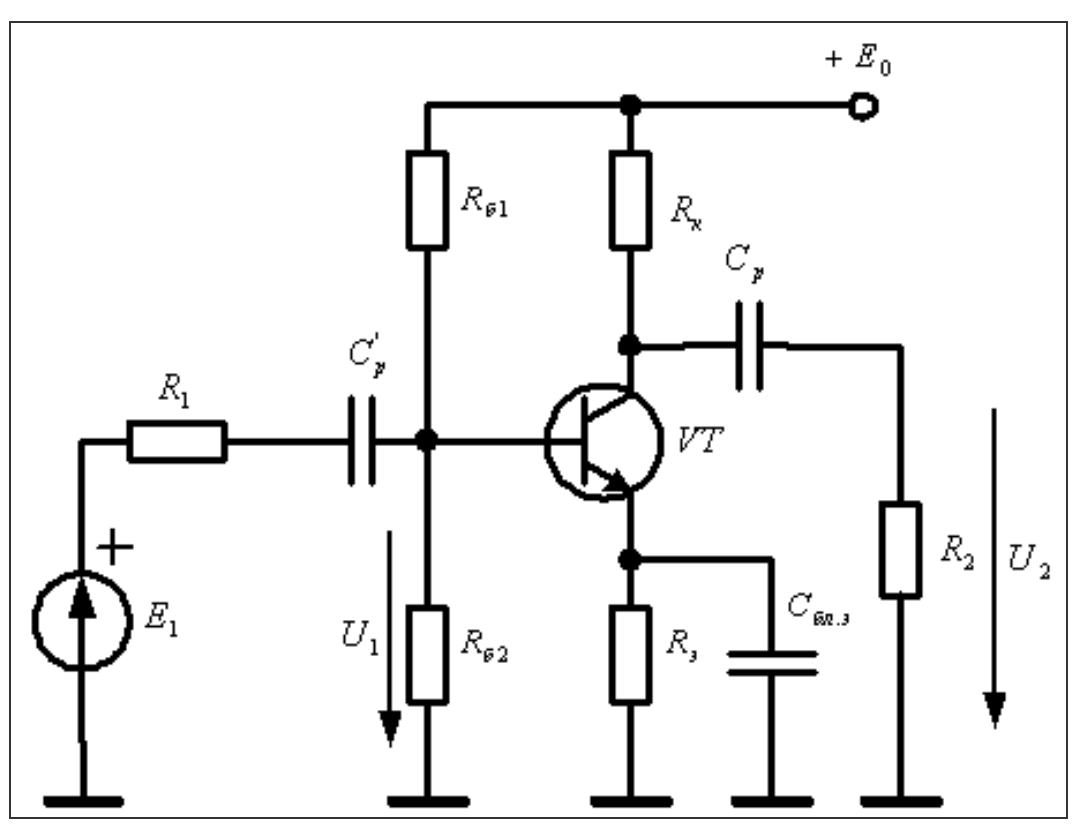
\includegraphics[scale=0.2]{oe.png}}
		\caption{каскад с ОЭ}
	\end{figure}
\end{center}

Эквивалентная схема:
\begin{center}
	\begin{figure}[h!]
		\center{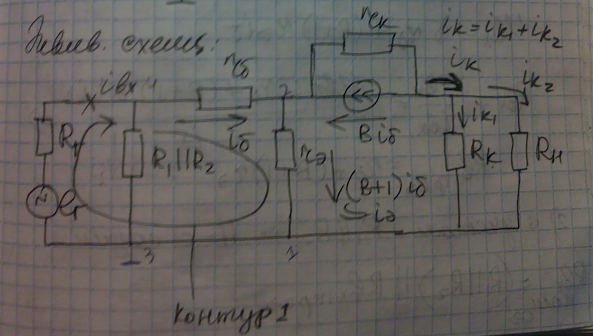
\includegraphics[scale=0.7]{oeekv.png}}
		\caption{эквивалентная схема с ОЭ}
	\end{figure}
\end{center}

1.Входное сопротивление:

$$R_{\textit{вх}}=\frac{U_{\textit{вх}}}{i_{\textit{вх}}}$$

$U_{\textit{вх}}= E_{\textit{г}} - i_{\textit{вх}}R_{\textit{вх}}$

1)Без $R_1 || R_2$, тогда $i_\textit{вх}=i_\textit{б}$

$U_{\textit{вх}}=\varphi_4-\varphi_3=i_\textit{б}r_\textit{б}+i_\textit{э}r_\textit{э}$
(контур 1 по закону Кирхгофа)

$i_{\textit{э}}=(B+1)i_\textit{б}$

$U_{\textit{вх}}=i_\textit{б}r_\textit{б}+(B+1)i\textit{б}r_\textit{э}$

$$
R_{\textit{вх}} = \frac{U_{\textit{вх}}}{i_{\textit{вх}}} = \frac{i_{\textit{б}}r_{\textit{б}} + (B+1)i_{\textit{б}}r_{\textit{э}} }{i_{\textit{б}}}
$$

$$
R_\textit{вхтроэ}=r_\textit{б} + (B+1)r_\textit{э}
$$

2)C учетом $R_1 || R_2$, получаем

$$
R_\textit{вх}=(R_1||R_2)R_\textit{вхтроэ}
$$

2. Выходное сопротивление:
 Выходное сопротивление определяется при отключении нагрущки и при нулевом входном сигнале
 
 $$R_\textit{вых}=\frac{U_\textit{хх}}{i_\textit{кз}}$$

$ U_\textit{хх}=I_\textit{к}R_\textit{к} $

$\frac{I_\textit{к}}{I_\textit{б}}=B,\Rightarrow U_\textit{хх}\approx BI_\textit{б}R_\textit{к}$

$$
I_\textit{кз}\approx BI_\textit{б},\Rightarrow R_\textit{выхоэ}=\frac{BI_\textit{б}R_\textit{к}}{BI_\textit{б}}
$$

3. Коэффициент передачи по напряжению:
$$
K_\textit{uоэ}=\frac{U_\textit{вых}}{U_\textit{вх}}=\frac{B(R_\textit{к}||R_\textit{н})}{R_\textit{вхтроэ}}
$$

4. Коэффициент передачи по току:

$$K_\textit{iоэ}=\frac{i_\textit{вых}}{i_\textit{вх}}=\frac{i_\textit{н}}{i_\textit{вх}}$$

$R_k \textit{ и } R_H$ включены параллельно $i_\textit{к}$ входит в $R_\textit{k}||R_\textit{Н}$

$$i_\textit{н}=i_\textit{к}\frac{R_\textit{к}}{R_\textit{н}+R_\textit{к}}$$

$i_\textit{вх}$ - ток через $[R_1||R_2]||R_\textit{вхтроэ}\Rightarrow$

$i_\textit{б}+i_{R_1R_2}=i_\textit{вх}$

$U_{R_1R_2}=U_\textit{вхтроэ}$

$i_{R_1R_2}[R_1||R_2]=i_\textit{б}R_\textit{вхтроэ}$

$i_{R_1R_2}=i_\textit{б}\frac{R_\textit{вхтроэ}}{R_1||R_2}$

$i_\textit{вх}=i_{R_1R_2}+i_\textit{б}=\left(\frac{R_\textit{вхтроэ}}{R_1||R_2}+1\right)i_\textit{б}$

$$K_i=i_k\frac{R_k}{R_k+R_H}\frac{1}{\left(\frac{R_\textit{вхтроэ}}{R_1||R_2}+1\right)i_\textit{б}}=B\frac{R_k}{R_k+R_H}\frac{R_1||R_2}{R_\textit{вхтроэ}+R_1||R_2}
$$

\pagebreak

